\documentclass{article}

\usepackage{ctex}
\usepackage{listings}
\usepackage[framed,numbered,autolinebreaks,useliterate]{mcode}
\usepackage{geometry}
\usepackage{multirow}
\usepackage{graphicx}
\usepackage{amsmath}
\usepackage{float}
\geometry{a4paper, scale=0.8}

\title{数学实验实验报告}
\author{ZhaohengLi 2017050025\\cainetatum@foxmail.com\\15801206130}

\begin{document}
\maketitle
\section{实验目的}
\begin{itemize}
	\item{掌握概率统计的基本概念;}
	\item{练习使用 MATLAB 解决实际概率问题。}
\end{itemize}


\section{CH11-T5 炮弹问题}
\subsection{算法设计}
设目标中心为$x=0,y=0$,记$a=100$,则圆形区域表示为:

$$\Omega:x^2+y^2\leq a^2$$

根据题目给出的炮弹落点的概率分布,可以得到:

$$p(x,y)=\frac{1}{2\pi\sigma_x\sigma_y\sqrt{1-r^2}}exp(-\frac{1}{2(1-r^2)}(\frac{x^2}{\sigma^2_x}-2r\frac{xy}{\sigma_x\sigma_y}+\frac{y^2}{\sigma^2_y}))$$

其中,$\sigma_x=80,\sigma_y=50,r=0.4$,则炮弹命中圆形区域的概率是二重积分:

$$P=\int\int_\Omega p(x,y)dxdy$$

实际计算的时候,去两个随机数X,Y均匀分布在$[-a,a]$上,则最终的数值计算公式为:

$$P=\int\int_\Omega p(x,y)dxdy\approx \frac{a^2}{n}\sum^m_{k=1}p(x_k,y_k)$$

其中m为n个随机点中落在$\Omega_1$中的点数。产生均匀分布的随机数可以采用MATLAB中的unifrnd函数实现。


\subsection{算法实现}

MATLAB代码实现如下:

\begin{lstlisting}
%% Global Variables
a = 100; sx = 80; sy = 60; r = 0.4; n = 10000;

%% Calculation
m = 0; z = 0;
x = unifrnd(−a, a, 1, n);
y = unifrnd(−a, a, 1, n);
for i = 1:n
	if x(i)^2 + y(i)^2 <= a^2
		u = 1 / (2 * pi * sx * sy * sqrt(1 − r^2)) * ...
			exp(−1 / (2 * (1− r^2)) * (x(i) * x(i) / (sx^2))− ...
    		2 * r * x(i) * y(i) / sx / sy + y(i) * y(i) / (sy^2));
		z = z + u;
		m = m + 1;
	end
end

%% Ans
P=a*a*z/n

\end{lstlisting}

\subsection{计算结果与分析}

通过使用不同的n值多次求解,得到如下计算结果:

\begin{figure}[H]
    \centering
    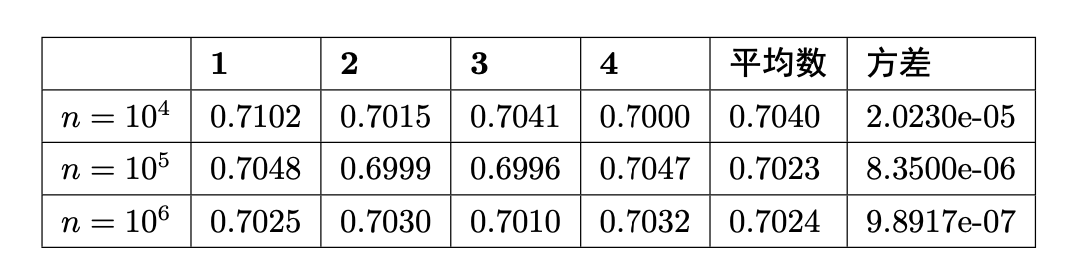
\includegraphics[width=0.6\textwidth]{pic1.png}
\end{figure}

首行的1,2,3,4分别为第1,2,3,4次计算的结果。

首先可以看出,随着 n 的增长,最终求得结果的方差不断减小,代表采样精度越高,得到的结果精确度也就相应地增加,符合辛钦定理内容和蒙特卡洛法相关结论。

另外可以看出最终结果都在 0.7 附近。

\subsection{结论}

根据计算精度进行估计,可以得出炮弹命中圆形区域的概率大概为 0.7。


\section{CH11-T7 报童问题}

\subsection{模型建立}

每天报纸的需求量为随机变量,记每天需求量为 r 的概率为 $f (r), r = 0, 1,\cdots. $。设报童 每天购进报纸份数为 n,根据课本问题 1的建模思路,可以得到报童每天的平均利润为:

$$V(n)=\sum^{n-1}_{r=0}[(b-a)r-(a-c)(n-r)]f(r)+\sum^\infty_{r=n}[(b-a)n]f(r)$$

将n和r看成连续变量,又有$a=a(n)=A(1-\frac nK)$,对$V(n)$求导可以得到:

$$V'(n)=\int^n_0[c-(a'(n)n+a(n))]p(x)dx+\int^\infty_n[b-(a'(n)n+a(n))]p(x)dx$$

带入$a'(n)n+a(n)=A(1-\frac{2n}{K})$,令$V'(n)=0$,则:

$$0=\int^n_0[c-A(1-\frac{2n}{K})]p(x)dx+\int^\infty_n[b-A(1-\frac{2n}{K})]p(x)dx$$

由题目数据可以知道,当均值比标准差大得多时,有:

$$\int^n_0p(x)dx\approx\int^n_{-\infty}p(x)dx$$

因此可以化简上式为:

$$\int^n_{-\infty}p(x)dx=\frac{b-A(1-\frac{2n}{K})}{b-c}$$

可以证明$V''(n)<0$,可以得到的n即为每天平均利润最大的最佳购进量。


\subsection{算法实现}

实际上,模型最终的式子是一个关于 n 的方程,不存在显式解,因此需要求解方程得到 最终的最优值。计算正态分布的时候可以采用 MATLAB 的 norminv函数,而求解方程组可 以采用 fzero函数。


\begin{lstlisting}
global K;
K = 50000;
kset = 25000:1000:800000;
vset = [];
for K = kset
    vset = [vset fzero(@news, [100, 3000])];
end
plot(kset, vset)


function [ y ] = news( x )
    mu = 2000;
	sigma = 50;
	A = 0.5;
	b = 0.5;
	c = 0.35;
	global K;
	target = (b − A * (1 − 2 * x / K)) / (b − c); y = norminv(target, mu, sigma) − x;
end

\end{lstlisting}

\subsection{计算结果与分析}

计算结果为:$1968.2$。

报童利润和参数 K 的曲线关系如下图所示,可以看出该参数越大,批发价下降得慢, 导致获得最大利润时卖出得报纸数目减少。

\begin{figure}[H]
    \centering
    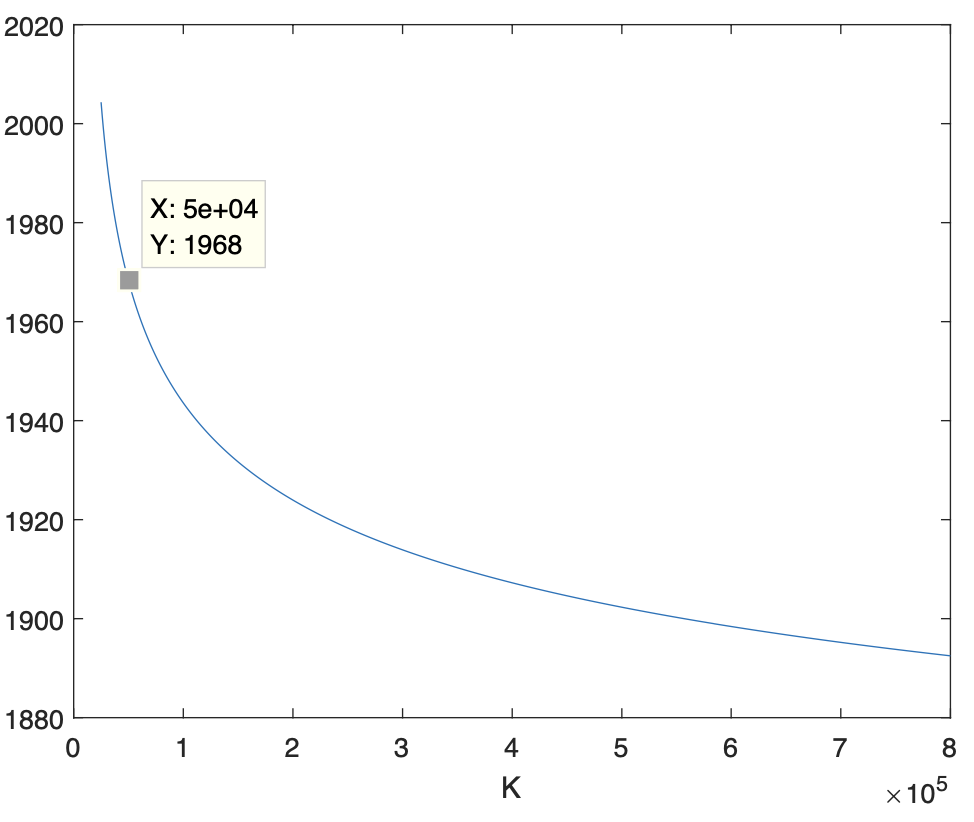
\includegraphics[width=0.4\textwidth]{pic2.png}
\end{figure}

另外考虑题目中给出得公式,显然在这种设定下购买的报纸越多,批发价就越便宜,且 线性关系带来的一个问题就是当 n 无限增大的时候,批发价会是负值,这个时候报童的期望 利润实际可以达到无穷,而这种情况是无法简单通过 $V''(n) = 0 $以及 $V''(n) < 0$ 捕获的。


\subsection{结论}

当报童每天卖出 1968 份报纸的时候,能够获得的期望利润最大。


\section{CH11-T9 轧钢问题}
\subsection{模型建立}

首先对问题进行简要的定性分析:如果轧钢设备所设定的平均长度过大,则精轧时切割 的长度也就越大,造成的浪费很多;而相反如果平均长度过小,则报废的可能性也增加,但 相应符合要求的那部份钢材会被精轧切割的长度也就越小,二者为相互制约的关系。因此对 于浪费问题需要权衡这里的参数 m,使得两种意义上的浪费最少。

设粗轧得到的钢材长度为随机变量 L,根据题意 $L\sim N (m, \sigma)$,其中 m 为可以控制的均 值,而 $\sigma$ 为不可控制的误差。

设 L 的概率密度函数为 $p(x)$,每粗轧一根钢材的期望浪费为 $W_1$,根据题意可以得到:

$$W_1=\int^\infty_1(x-l)p(x)dx+\int^l_{-\infty}xp(x)dx$$

上式由两部分组成,一部分为整根报废的浪费量,另一部分为精轧时的浪费量。进一步 化简为:

$$W_1=\int^{\infty}_{-\infty}xp(x)dx-l\int^{\infty}_1p(x)dx=m-l\int^\infty_1p(x)dx=m-lP$$

其中$P=\int^\infty_1p(x)dx$,意义是粗轧钢材长度大于 l 的概率,同时也代表了最终能够得到l规定长度钢材(而不是整根报废)的概率。

因此,最终需要优化的值即为:

当目标函数为每粗轧一根钢材浪费最小时,目标函数即为 $W_1 = m − lP$。

当目标函数为每得到一根规定长度钢材浪费最小时,目标函数为 $W_2 = \frac{W_1}{P} = \frac mP − l$。


\subsection{算法实现}

MATLAB代码实现:

\begin{lstlisting}
global sigma;
global l;
sigma = 0.2;
l = 2;

fminbnd(@w1, 2, 3)

fminbnd(@w2, 2, 3)

function [ y ] = w1( m )
    global l;
	global sigma;
	P = (1 − normcdf(l, m, sigma)); y = m − l * P;
end

function [ y ] = w2( m )
    global l;
	global sigma;
	P = (1 − normcdf(l, m, sigma)); y = m ./ P − l;
end

\end{lstlisting}

\subsection{计算结果与分析}
MATLAB 的输出依次为 2.3327和 2.3562。此外,可以绘制出函数 $W_1$ 和 $W_2$ 随 m 变 化如下图所示。

\begin{figure}[H]
    \centering
    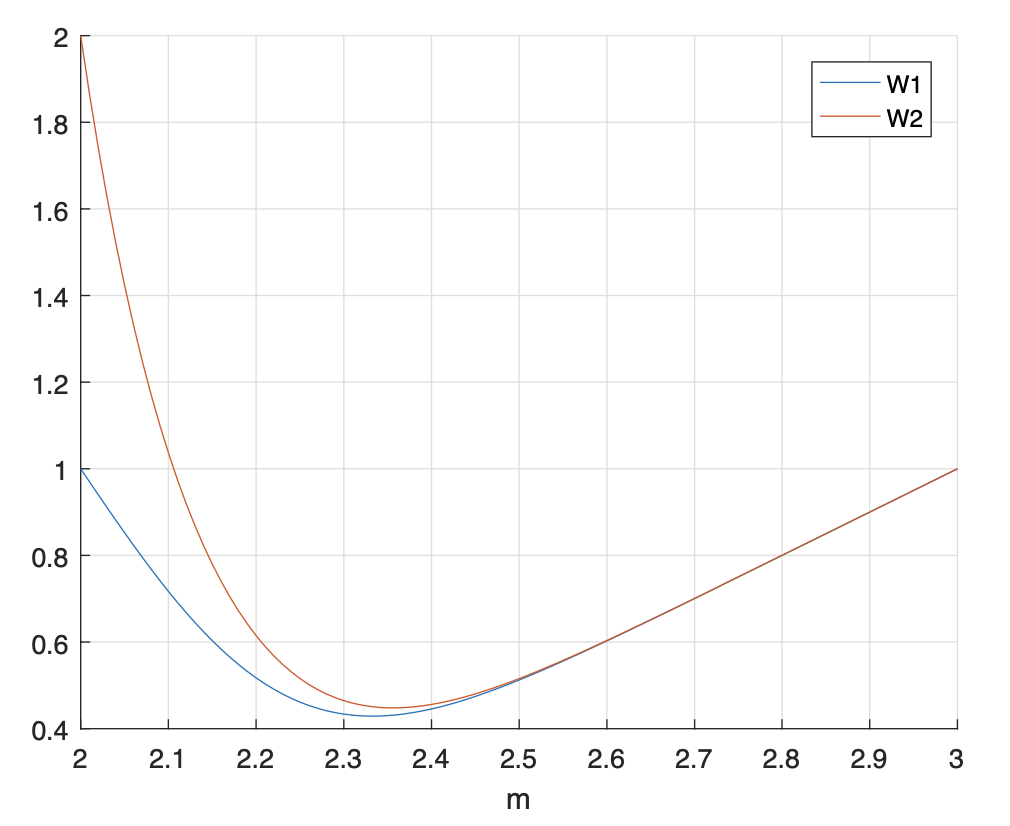
\includegraphics[width=0.4\textwidth]{pic3.png}
\end{figure}

从图中能够看出,当 m 减小时,两种浪费均增加,这体现在报废钢管数目的增加上;当 m 增大时,浪费也增加,这体现在精轧过程中的截取更多。但是对比 $W_1$ 和 $W_2$,当 m 减小 的时候,$W_2$ 增加的更加显著,这是因为规定长度钢材的总数目越来越少,合格率越来越低, 如果这个代价分摊到所有合格的钢管上,平均浪费显然会更高一些。另外,随着 m 的增高, 报废率越来越少,两种浪费的计量数值也会越来越接近。


\subsection{结论}

当目标函数为每粗轧一根钢材的浪费最小时,m = 2.33m;

当目标函数为每得到一根规定长度钢材浪费最小时,m = 2.36m。


\section{实验总结}

通过这次的实验,我学会了使用 MATLAB 求解统计问题的一般方法,并对概率论与数 理统计的知识有了更深的理解。希望在之后的课堂上老师能够当堂进行相关的技巧演示并给 出题目的分步解答。


\end{document}